%===============================================================
% ICCAD 2014 submission
%
% ===============================================================

\documentclass[10pt,nocopyrightspace]{sigplanconf}

\usepackage{multirow}
\usepackage{amsthm}
\usepackage{amsmath}
\usepackage{amssymb}
\usepackage{empheq}
\usepackage{algorithm}
\usepackage[vlined,linesnumbered,ruled,algo2e]{algorithm2e}
\usepackage{color}
%\usepackage{subfigure}
\usepackage{subcaption}
\usepackage{booktabs}
\usepackage{url}
\usepackage[normalem]{ulem}
%\usepackage{subfig}
\usepackage{verbatim}
%\usepackage{listings}
\usepackage[caption=false,labelformat=simple]{subfig}
\usepackage{flushend}
\usepackage{paralist}
\usepackage{array}
\usepackage{enumitem}

\usepackage[compact]{titlesec}
\setlength\extrarowheight{1pt} % or whatever amount is appropriate

\newcommand{\fixme}[1]{\textcolor{red}{\small [~#1~]}}
\newcommand{\TT}[1]{\texttt{#1}}
\newcommand{\BF}[1]{\textbf{#1}}
\newcommand{\IT}[1]{\textit{#1}}
\newcommand{\RM}[1]{\textrm{#1}}
\newtheorem{lemma}{Lemma}
\newtheorem{theorem}{Theorem}

\newcommand{\interval}{T}
\newcommand{\latency}{L}

%%%%%%%%%%%%%%%%%%%%%%%%%%%%%%%%%%%%%%%%%%%%%%%%%%
\begin{document}
\renewcommand{\thesubfigure}{(\alph{subfigure})}
\title{ECE 5770 : Resilient Computer Systems \\
Modeling On-Die Termination Power Overhead of Encrypted Data}

\authorinfo{Udit Gupta, Monica J. Lin}
{School of Electrical and Computer Engineering, Cornell University, Ithaca, NY}
{ug28@cornell.edu, mjl256@cornell.edu}

\maketitle

\begin{abstract}
\label{sec-abstract}
%A short summary of the paper
As the number and heterogeneity of computing devices steadily
increases, it becomes more crucial for hardware and software designers to
provide security primitives to users. Each day, these devices communicate
countless pieces of sensitive data that must be adequately protected. The need
to maintain the confidentiality of memory is just one aspect of this security
problem, as it safeguards a user's information. Recent research efforts have
focused on developing cryptographic memory encryption primitives for the
general purpose and high performance computing domains however mobile and
embedded devices pose an interesting challenge with strict first-order power
constraints. This study focuses on modeling the effect of memory encryption on
off-chip memory power consumption by focusing on the effects of link
termination and signal reflections that arise when driving Data-Bus Inversion
(DBI) enabled DDR4 memory technologies. Using MiBench, a set of applications
representative of mobile workloads, and Pin, a computer architectural
simulator, we find that memory encryption does incur a significant power
overhead. We provide a framework for users to run arbitrary binary executables,
specify first-level cache configurations and analyze DBI ratios of secure
memory systems with encryption and insecure memory systems without encryption.
\end{abstract}

\section{Introduction}
\label{sec-introduction}

%Define the problem and the goal of the project
%Explain why the problem is important
%Summarize your approach and key results
%Outline the rest of the paper

Since the advent of the Internet, computing devices have become not only more
prolific but also more varied - encompassing not only high performance
clusters but also general purpose computers and mobile systems.  Moreover, the
assumptions made about the security model of a system have changed drastically;
users can no longer be trusted, and devices have the potential to interact with
unknown and possibly untrustworthy hosts while communicating sensitive
information. For example, the boom in smartphones has caused a secondary
explosion in the mobile application industry, allowing users to log in to
various trusted systems (e.g. bank accounts, medical records and shopping
accounts) remotely.  The sudden increase in connectivity exposes users to
adversaries that may attempt to leverage these interactions in order to obtain
confidential information or disrupt the use of services or applications.

In response to these changes, there has been an increasing effort in developing
trusted computing platforms augmented with specialized hardware modules that
provide security features such as authentication and decryption/encryption. One
such security feature that remains a focus in trusted computing research is
protecting off-chip memory. One key component of protecting off-chip memory is
maintaining confidentiality of private data. Challenges in designing memory
protection mechanisms involves providing encryption primitives at a low cost
(money, area, power and design complexity), high throughput and low latency
without compromising security. Current work also focuses on memory protection
schemes for general purpose and high performance computing systems. The domain
of memory protection in the mobile and embedded computing domains is relatively
less studied and poses interesting challenges. Mobile and embedded devices
often operate under strict power and area constraints. Providing secure memory
protection while following the prescribed power and area constraints as well as
maintaining performance of the computing devices is an ongoing challenge.

According to Hollis \cite{hollis} there are two main source of power
consumption when driving I/O:

\paragraph{Dynamic A/C Power} Dynamic A/C power consumption from charging and
discharging capacitances (e.g. electrostatic discharge devices, driver output
capacitance, receiver input capacitance and the channel itself), is possibly
the dominant and most universal form of I/O power consumption. However, once
the capacitances have reached steady state, the dynamic a/c power consumption
is negligible. For the purposes of our study we assume that all device
capacitances are already in steady state - simplifying our model as we no
longer have to consider dynamic a/c power consumption.

\paragraph{Link Termination} The second most common source of I/O power
consumption is link termination schemes. Intuitively, when the driver
outputs a signal which is then received by the I/O device, a significant
portion of the signal is reflected back to the driver itself. Consequently, the
driver has to not only power the desired signal but also overcome the signal
reflections.  This incurs a significant power overhead. Past research in the
context of link termination schemes has focused on developing more efficient
DDR chip topologies to reduce signal reflections. For example, in Figure
\ref{dram-chips} illustrates the DDR2 and DDR3 DDR chip topologies. As driving
frequencies for DDR3 increased, memory architects adopted the fly-by network
topology which greatly reduces signal reflections and improves On-Die
Termination (ODT).

\begin{figure}[!htb]
  \centering
  \begin{subfigure}[b]{0.4\textwidth}
    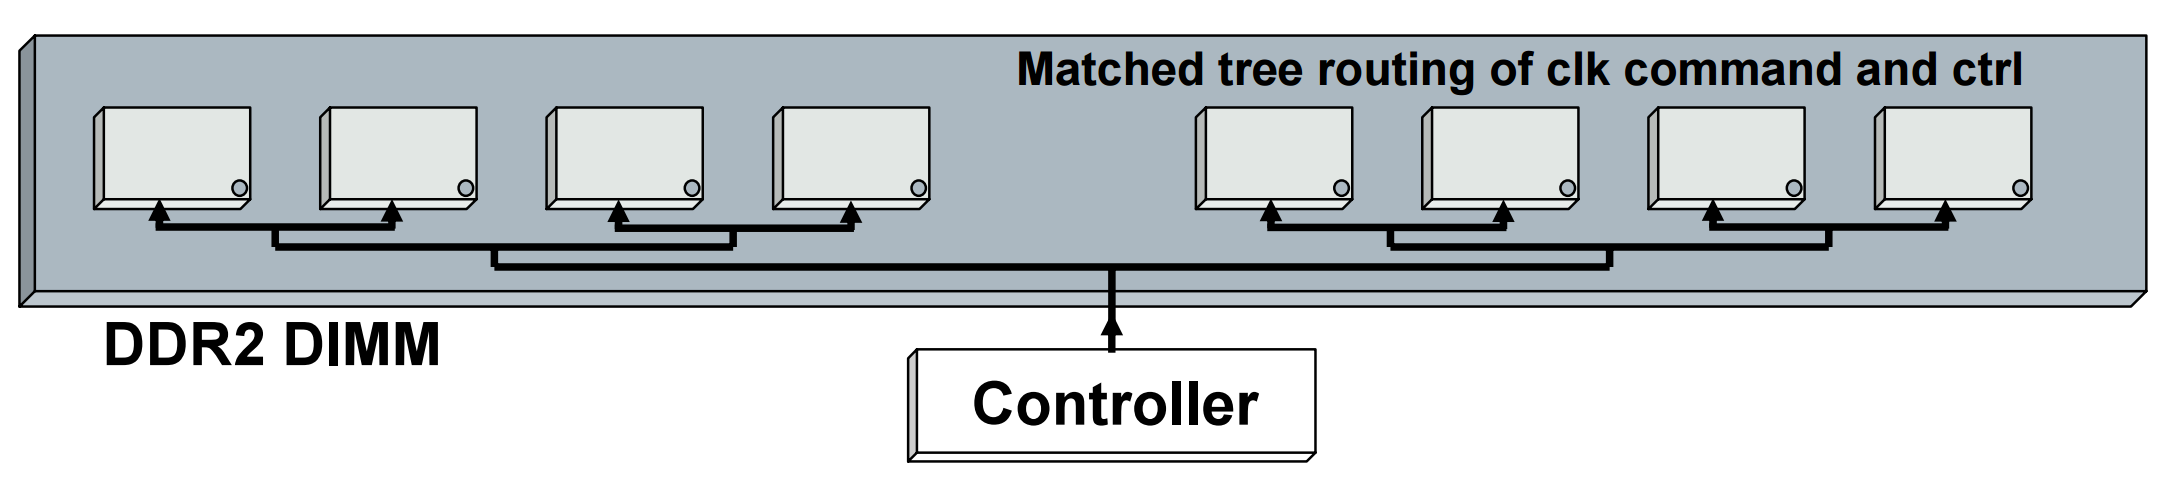
\includegraphics[width=\textwidth]{figs/ddr2-topology}
    \caption{Example DDR2 DRAM chip topology}
    \label{fig:ddr2-chips}
  \end{subfigure}

  \begin{subfigure}[b]{0.4\textwidth}
    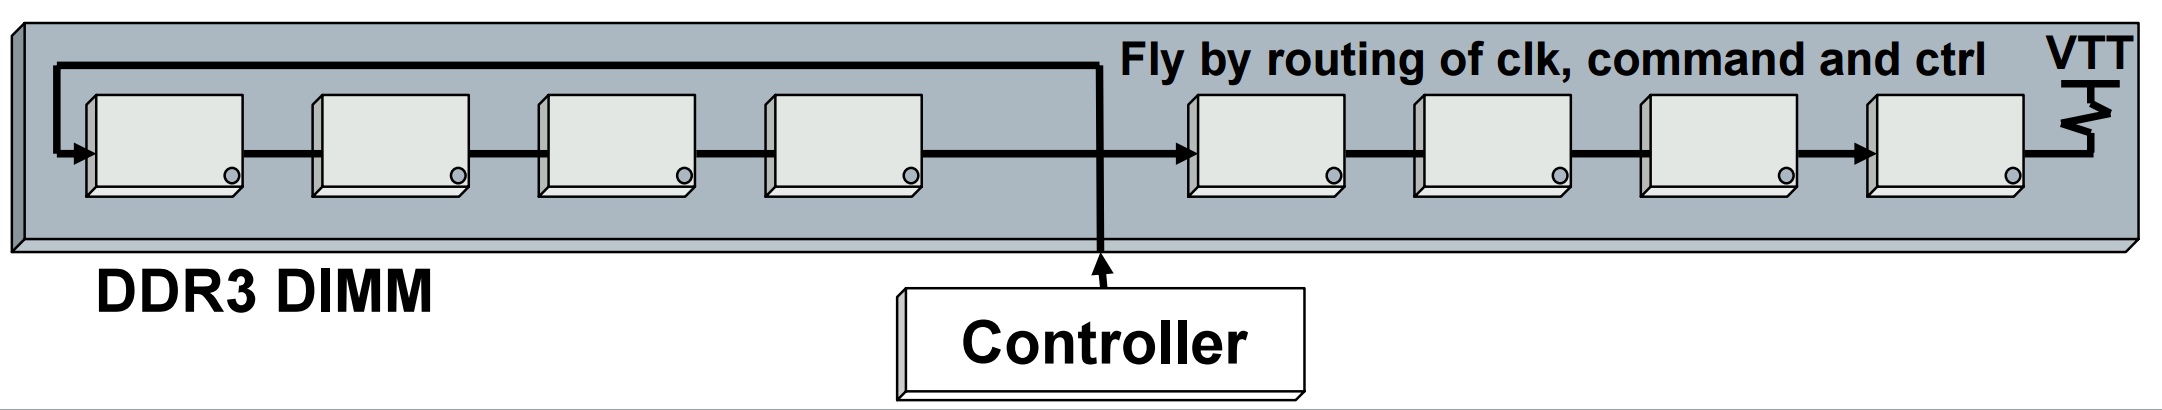
\includegraphics[width=\textwidth]{figs/ddr3-topology}
    \caption{Example DDR3 DRAM chip topology}
    \label{fig:ddr3-chips}
  \end{subfigure}
  \caption{Representative DRAM chip topologies for DDR2 and DDR3 memory
  technologies taken from \cite{ddr-design}}
  \label{dram-chips}
\end{figure}

Though existing DDR3 memory technologies implement more efficient DRAM chip
topologies to reduce signal reflections, ODT is still a prominent source of
power consumption. Memory architects are looking at more efficient read/write
schemes such as Data Bus Inversion (DBI) for further improving ODT power
consumption for DDR4. Our study focuses on using first order models for DBI
developed by Hollis \cite{hollis} in the context of memory encryption to
simulate the power overhead of secure memory encryption. Generally, our results
so that memory encryption does indeed incur a significant power overhead and
that DBI-DC and AC values for is relatively consistent across MiBench
applications.

The rest of this paper is organized as follows: Section~\ref{sec-problem}
outlines our general project goals and outlines the memory encryption model
used, Section~\ref{sec-methodology} outlines the high level model and
experimental setup for our study, Section~\ref{sec-evaluation} analyzes our
results and data, Section~\ref{sec-group-dynamics} reviews our group dynamic's
and work distribution, Section~\ref{sec-related} reviews related work in
relation to power consumption of secure memory encryption and
Section~\ref{sec-conclusions} concludes the paper with final remarks and future
work.

\section{Problem Formulation}
\label{sec-problem}

%Describe the problem that you are trying to solve, or the application that you
%are trying to implement

Figure \ref{fig:sys-arch} illustrates the general secure memory encryption
architecture used in this study. The threat model assumes that the
on-chip memory, \TT{data-cache}, is secure and tamper-proof whereas the
off-chip memory is not. The \TT{encryption core} between the data-cache is
supposed to provide cryptographic confidentiality properties that prevent
unauthorized principals from reading sensitive information that user's wish to
keep secret.

\begin{figure}[!htb]
  \centering
  \includegraphics[width=0.5\textwidth]{figs/sys-arch}
  \caption{General Memory Encryption Architecture: All on-chip memory accesses,
  between the processor and data-cache, are performed in plaintext whereas all
  off-chip, between the data-cache and DRAM, are encrypted.}
  \label{fig:sys-arch}
\end{figure}

Typically, the encryption core seen in Figure \ref{fig:sys-arch} implements the
\TT{AES-CTR} mode scheme.  Where previous studies have focused on the
performance and area overhead of memory encryption, we wish to explore the
impact of memory encryption on the power consumption of off-chip memory storage
systems. Specifically we want use various computer architecture analysis tools
to simulate memory access traces and model the power overhead of encryption on
DDR4 memory technology. Our first order model characterizes the \TT{ODT} power
overhead when using \TT{Data-Bus Inversion} for realisitic benchmarks
targetting mobile systems using DDR4 memory technology.

\section{Methodology}
\label{sec-methodology}

%Describe your approach and design
%Instead of simply explaining what you ended up doing, show why you made such
%design decisions / how what the trade-offs are.

As mentioned earlier, DRAM power consumption is dominated by
charging/discharging chip capacitances and signal reflections caused by link
terminations. Once the capacitors have reached steady state, their power
consumption is negligible in comparison to the system as a whole and thus can
be neglected from our power models. Instead we focus on link termination and
signal reflections. Specifically, DDR4 memory technology leverages \TT{DBI} to
reduce the signal reflections and power consumption. Intuitively, DBI aims to
reduce the number of bit flips (DBI-AC) and binary signal probabilities
(DBI-DC) to improve power consumption of read and write operations. For
reducing bit flips, take for example the case where memory location $M$
previously had the value $00000000$ that was being overwritten by the value
$11111111$. Instead of flipping every bit in $M$, a DBI-AC enabled memory system
would retain the previous state of $00000000$ and set the DBI flag that
signifies that all the bits are flipped.  This would incur the power consumption
of 1 bit flip, not the entire data byte.  Since the power consumption of 0 and
1 is not the same, depending on memory technology constraints, DBI-DC aims to
reduce the prevalence of the higher power consuming bit. In the case of DDR4,
$0$ consumes more power and thus DBI aims to reduce the number of $0$'s and
increase the number of $1$'s \fixme{add citation}. Figure \ref{fig:dbi-dc}
illustrates the impact of DBI-DC on improving signal quality and consequently
power consumption of read and write operations. The larger open data eye
illustrates that there is less interference between the driver and reflected
signals when using DBI-DC and the smaller $V_{pp}$ suggests that the driver has
to work less with DBI-DC enabled.

\begin{figure}[!htb]
  \centering
  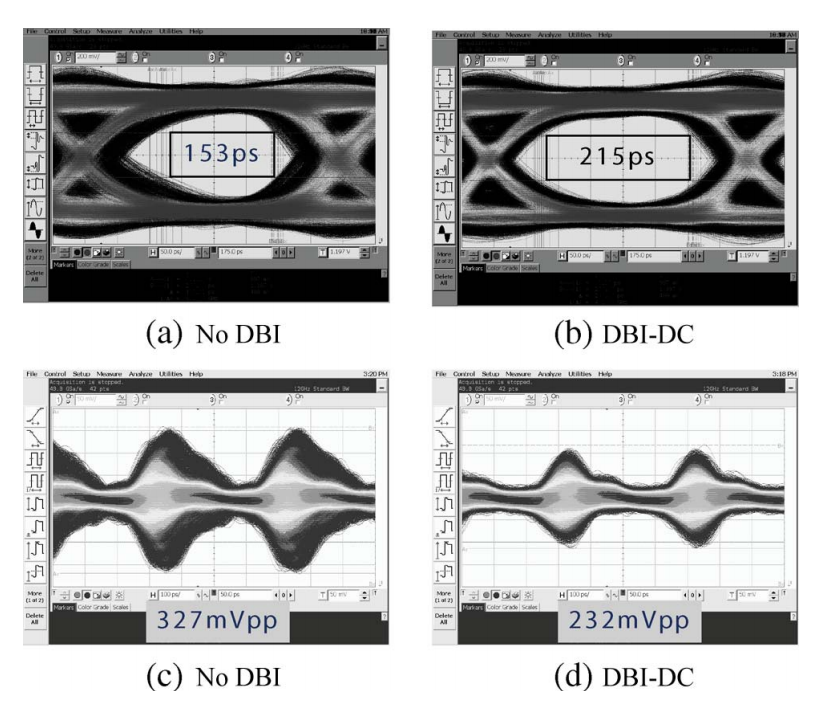
\includegraphics[width=0.3\textwidth]{figs/dbi-dc}
  \caption{Using DBI-DC increases the open data eye and reduces the required
  $V_{pp}$ for effectively driving the DRAM chip. Taken from \cite{hollis}}
  \label{fig:dbi-dc}
\end{figure}

The following sections outline our model, and experimental setup for measuring
the ODT power overhead of memory encryption on DBI-enabled DDR4 memory
technology.

\subsection{Model}
In order to model the power overhead of memory encryption on DBI-enabled memory
technologies, we use the same model described by Hollis \cite{hollis}, shown
below:

    $$ P_t = A \times P_{dc} + B \times P_{ac}$$

Where $P_t$ is the ODT power consumption, $P_{dc}$ is the intrinsic DC-power
consumed and $P_{ac}$ is the intrinsic AC-power consumed by bit flips. The
ratios $A$ and $B$ determine the DC and AC factors of $P_t$ respectively.
DBI-DC aims to exploit program structure and reduce $A$ whereas DBI-AC aims to
reduce $B$. Together they can significantly decrease the ODT power consumption.
As Hollis \cite{hollis} describes - under the assumption that data written to
memory or read from memory are completely random:

  $$ A = 0.5$$
  $$ B = 0.5$$

Intuitively, truly random data would have equal probability of each binary
digit making $A = 0.5$. Similarly, truly random data would have equal
probability of flipping or not flipping and thus, $B = 0.5$. In order to model
ODT power consumption, we must determine the values of $A$ and $B$ for secure
memory systems with encryption and insecure memory systems without encryption.
The following sections outline our experimental setup for analyzing the DBI
enabled power model described.

\subsection{Experimental Setup}

\begin{figure}[!htb]
  \centering
  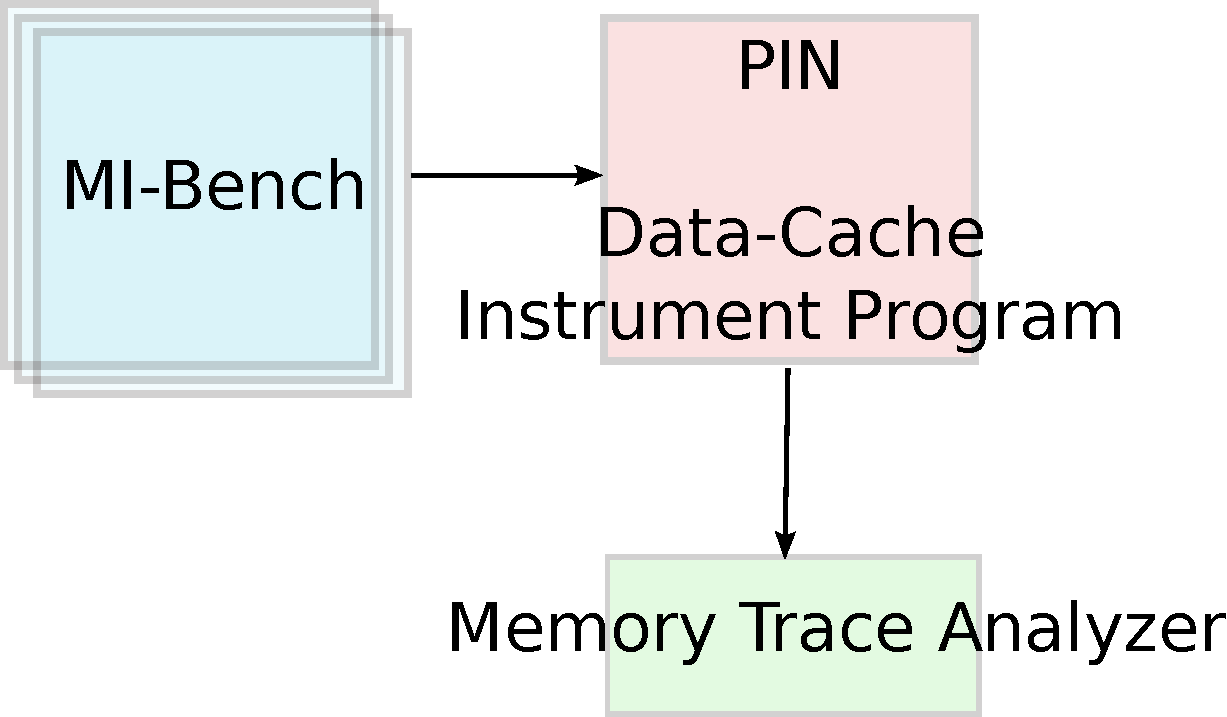
\includegraphics[width=0.3\textwidth]{figs/exp-design}
  \caption{General system architecture for the experimental setup for analyzing
  the DBI enabled power model}
  \label{fig:exp}
\end{figure}

Figure \ref{fig:exp} illustrates the general experimental setup we used to
implement the DBI model described earlier. First, we need a set of
representative benchmarks to run through to generate realistic memory traces
that can be used to analyze the effect of memory encryption on power
consumption. We chose MiBench \cite{mibench} for our benchmark suite. MiBench
consists of applications representative of embedded and mobile workloads and
provides easy to use build binary executables which integrates well with the
\TT{PIN} architectural simulator we used. We chose not to use the \TT{SPEC2006}
benchmark as the applications targeted workloads handled by general purpose
processors. We used 28 applications in the MiBench suite (the following 14
applications on big and small data-sets):

\begin{multicols}{2}
  \centering
  \begin{enumerate}
    \item \TT{basicmath}
    \item \TT{bitcount}
    \item \TT{qsort}
    \item \TT{susan}
    \item \TT{jpeg}
    \item \TT{dijkstra}
    \item \TT{patricia}
    \item \TT{stringsearch}
    \item \TT{blowfish}
    \item \TT{sha}
    \item \TT{adpcm}
    \item \TT{CRC32}
    \item \TT{FFT}
    \item \TT{gsm}
  \end{enumerate}
\end{multicols}

The chosen set of MiBench applications spans all six classes provided by the
benchmark: \TT{automotive}, \TT{consumer}, \TT{network}, \TT{office},
\TT{security}, and \TT{telecomm}.

\subsection{Architectural Simulator}

\begin{enumerate}
  \item PIN - dynamic binary instrumentaiton tool : describe cache settings
  \item Computer architecture analysis tool
  \item DRAMSim - Did not work for us.
  \item Python Script to analyze the loads and stores from the trace outptted
    from PIN
\end{enumerate}

\section{Evaluation}
\label{sec-evaluation}

%Metrics: what do you care about?
%Evaluation methodology: how did you evaluate?
%Results / discussions: if possible, provide intuitions and reasons for the
%result you got.

As described in the previous section, our study focuses on analyzing the AC and
DC power consumption ratios. Intuitively we would expect that DBI-AC and DBI-DC
help the AC and DC power consumption factors respectively. Table
\ref{table:dbi-ratios} illustrates the AC and DC ratio reductions for load and
store operations separately. The average ac/dc ratio improvements were computed
using the following formula:

$$ \TT{\% Improvement} = |\frac{\TT{DbiRatio} - \TT{nonDbiRatio}}{\TT{nonDbiRatio}}| \times 100\%$$

\begin{table}[!htb]
  \centering
    \begin{tabular}{| c | c |}
      \hline
      \textbf{DBI Ratio} & \textbf{\% Improvement} \\ \hline
     Load DC  & 68.59 \\ \hline
     Load AC  & 8.62  \\ \hline
     Store DC & 75.04 \\ \hline
     Store AC & 3.38  \\ \hline
    \end{tabular}
    \caption{Average AC/DC ratio reduction for load and store operations using
    DBI across all 28 MiBench applications}
    \label{table:dbi-ratios}
\end{table}

We can see the DBI-DC reduces the DC factor by 68.6 \% and 75.0 \% for load and
store operations whereas DBI-AC has a smaller reduction of 8.6 \%
and 3.4 \% respectively. Since the DC factor optimized the data values to
reduce the number of binary $0$'s \cite{low-power-dram}, we can conclude that
the values on cache misses for both load and store operations were
predominantly $0$'s  in the MiBench suite. This suggests that DBI, especially
DBI-DC does indeed improve the AC and DC power consumption ratios for
unencrypted memory systems. Next we compare DBI's impact on unencrypted versus
encrypted memory systems.

\begin{figure}[!htb]
  \centering
  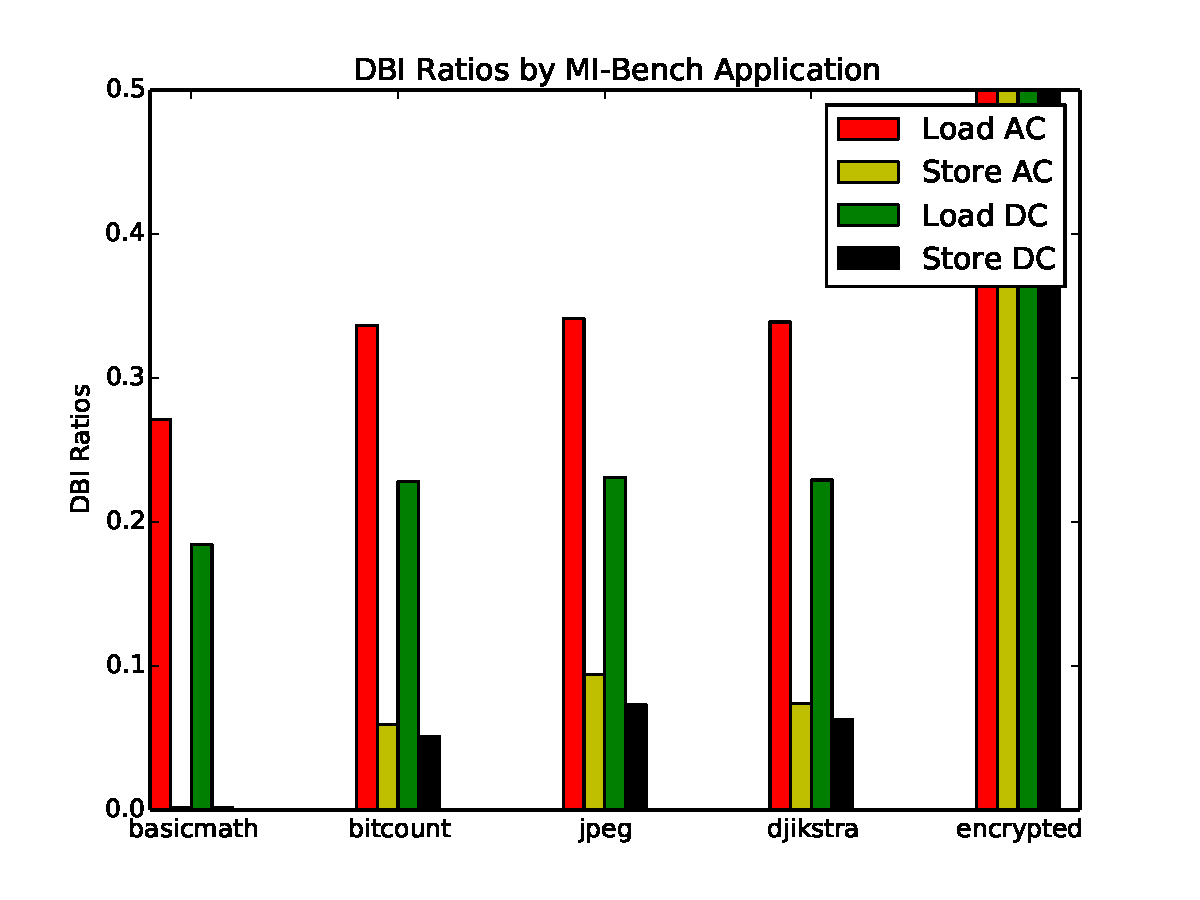
\includegraphics[width=0.5\textwidth]{figs/dbiGraph}
  \caption{Comparing load/store DBI ratios for representative MiBench applications}
  \label{fig:dbiGraph}
\end{figure}

Figure \ref{fig:dbiGraph} illustrates the DBI-AC and DBI-DC ratios for select
MiBench applications and our encrypted system model. The MiBench applications
chosen: \TT{basicmath}, \TT{jpeg}, \TT{djikstra}, \TT{fft}, \TT{bitcount},
\TT{blowfish}, and \TT{strsearch} span all six application classes of MiBench:
\TT{automotive}, \TT{consumer}, \TT{security}, \TT{office}, \TT{telecomm} and
\TT{network}. We chose these specific applications as they span all six
application classes of MiBench and are representative of the memory access
patterns for each of their domains.

\paragraph{Encryption Model} First, the encryption model exhibited DBI-AC and
DBI-DC ratios of 0.5 for both loads and stores. As mentioned in
Section~\ref{sec-methodology}, truly random data exhibits DBI-AC and DBI-DC
ratios of 0.5 \cite{hollis} since truly random data has equal signal
probabilities of 0 and 1, and equal switching probabilities (flip or not flip).
According to the Avalanche effect, changing even a single bit in the
unencrypted plaintext should cause the encrypted ciphertext to appear
completely random \cite{avalance}. Under the avalance effect, we assume
encrypted data is truly random for the purposes of this study. Furthermore, as
shown in Figure \ref{fig:sys-arch}, all cache misses are first encrypted with
the \TT{Encryption Core} before being processed by the off-chip DRAM based
memory system. This means that for the encrypted model, all data seen by the
DDR4 DRAM memory system will be truly random and DBI-AC and DBI-DC ratios will
be 0.5. Though the true DBI-AC and DBI-DC ratios may be less than 0.5, we
believe that the difference would not be significant enough to change the
underlying results of this study.

As seen in Figure \ref{fig:dbiGraph}, the DBI-AC and DBI-DC ratios for load and
store operations for the MiBench applications is significantly lower than that
of encrypted model. This suggests that for unencrypted data stores and loads
that follow the MiBench memory access pattern, DBI-AC and DBI-DC can
significantly reduce the AC and DC power factors to 0.33 for Load-AC,
0.07 for Store-AC, 0.22 for Load-DC and 0.06 for Store-DC on average across all
MiBench applications. If the encryption scheme seen in Figure
\ref{fig:sys-arch} were used, the DBI-AC and DBI-DC ratios would be 0.5. This
suggests that for load and store operations, encryption would incur a
significant power overhead.

Interestingly, we see that for all MiBench applications --- especially the
select ones shown in Figure \ref{fig:dbiGraph} --- the load and store ratios
are relatively consistent. This can be explained by the fact that for the given
cache architecture, the MiBench applications may have similar miss rates per
1000 instructions \cite{mibench}. From the select applications, \TT{rijindael}
and \TT{ispell}, and the given cache configuration : 32KB size, 8 way
associative and 128B cache lines both applications have around 3 misses per
1000 instructions. Assuming that the trend continues for the all applications
in the MiBench suite, the DBI ratio similarity across the applications is
expected. Furthermore, it should be noted that MiBench is organized such that
each application has two version: \TT{small-input} and \TT{large-input}. We
noticed that for all applications, the small and large input version exhibited
virtually the same DBI ratios which can also be explained by the fact that
despite the varying input data sets, the memory access pattern should be the
same across both versions resulting in similar DBI ratios.

\section{Group Dynamics}
\label{sec-group-dynamics}

%Describe contributions by each group member / how was the work split between
%the two.
Generally, we worked together for all parts of the project. To start with, we
came up with the design and overall experiment together. This included
investigating Gem5, SESC, and Pin. Since Monica had more experience regarding
the computer architectural simulators she was able to better understand the
benefits of using Pin versus Gem5 and ESESC. Next we split up the work for
getting Pin setup, acquiring benchmarks and investigating DRAM simulators.
Monica worked on acquiring the benchmarks and finding DRAM simulators - namely
DRAMSim. Udit worked on organizing, understanding and implementing a working
Pintool for generating the memory trace. Once the initial Pintool for
generating a memory trace using the \TT{pinatrace} and \TT{safecopy} examples,
(without a data-cache) was completed, we worked together to test the Pintool on
small generic \TT{bash} commands and sample programs we wrote.

The two of us then worked together on understanding DRAMSim and understanding
how to run the infrastructure using user inputted memory traces. After a few
days of analyzing the tool flow, the generated power traces, and the source
code we decided that DRAMSim would not be a viable option for our
project. At this point we went back to existing literature to find simple DBI
models for power modeling. This is when we found Hollis' model \cite{hollis}
and agreed to use it for our study. Concurrently we worked on implementing a
data-cache instrumentation tool using Pin to isolate the cache misses from all
memory accesses - a more realistic configuration for our project. Finally, once
the DBI model was decided, Udit focused on writing the simple Python script to
analyze the memory traces and Monica focused on organizing all of our sources,
background research and began working on the power-point presentation.

Needless to say, most of the project was done together since much of the work
was understanding existing models and tools.

\section{Related Work}
\label{sec-related}

We organize the related work surrounding efficient, low-cost memory protection
techniques in two separate sections : \textbf{memory encryption} and
\textbf{memory integrity verification}.

\subsection{Memory Encryption}
The goal of memory encryption techniques is to protect the confidentiality of
sensitive information from unauthorized subjects. Sensitive information
includes : secret keys, secret code (e.g. proprietary boot code) and private
data. The \TT{National Institute of Standards and Technology} (NIST) actively
regulates the encryption standards. Recently, two symmetric key cryptographic
algorithms are being increasingly used in trusted computing : Triple Data
Encryption Standard (3DES) and Advanced Encryption Standard/Rjindael (AES). As
AES provides systems with a higher minimum security strength, it is more widely
used in recent hardware accelerated trusted computing studies as compared to
3DES. For instance, Intel has developed extensions to it's instruction set
architecture (ISA) to enable fast encryption and decryption using AES. The
studies in this survey focus on using AES to develop efficient, low-cost
encryption and decryption modules.

%%%%%%%%%%%%%%%%%%%%%%%%%%%%%%%%%%%%%%%%%%%
\subsubsection{AES Counter Mode Encryption}
%%%%%%%%%%%%%%%%%%%%%%%%%%%%%%%%%%%%%%%%%%%
AES supports three general modes of operation: Electronic Codebook (ECB),
Cipher Block Chaining (CBC) and Counter (CTR). Since the AES-ECB mode preserves
patterns from the plaintext to the ciphertext, it does not provide adequate
confidentiality protection. Both AES-CBC and AES-CTR eliminate this information
leak by chaining the encryption between blocks. This however precludes users
from encrypting and decrypting blocks in parallel (as supported by AES-ECB). As
discussed in \cite{suh-memIntEnc}, decrypting the ciphertext stored in memory
can drastically increase the load use delay latency of processing systems. The
added latency is a result of the serial : fetch memory then decrypt memory
block operation. To hide this latency Suh et. al. use a \TT{one-time pad} (OTP)
based encryption / decryption technique. The OTP is generated by encrypting the
plaintext = {\TT{FV} $||$ \TT{Addr} $||$ \TT{TS} $||$ \TT{i}}, under a secret
key using AES-CTR. \TT{FV} is a fixed vector, \TT{Addr} is the memory address
being accessed, \TT{TS} is a timestamp stored along with the encrypted data and
\TT{i} is the block number. The use of a monotonically incrementing counter,
\TT{TS}, ensures the uniqueness of the \TT{OTP} which is then proven to be
secure. Generating the \TT{OTP} using this method enables the system to overlap
the AES-CTR decryption latency with the memory fetch / accessing latency
\cite{suh-memIntEnc}. Suh et. al. also mentions the \TT{TS} values can be
cached to mitigate the memory access latency for fetching the \TT{TS} and
better hiding the AES-CTR decryption latency. This method reduces the
load-use-delay latency to the latency of performing an $\oplus$ between the
generated \TT{OTP} and encrypted data.

%%%%%%%%%%%%%%%%%%%%%%%%%%%%%%%%%%%%%%%%%%%
\subsubsection{AEGIS}
%%%%%%%%%%%%%%%%%%%%%%%%%%%%%%%%%%%%%%%%%%%
Furthering the AES-CTR based decryption \cite{suh-memIntEnc}, AEGIS
\cite{aegis} adds low-level OS-kernel support to provide additional
confidentiality features. AEGIS, a single-chip secure processor, leverages
OS-kernel modes to provide additional encryption (ME mode) and
integrity-verification (IV mode) features. The OS also manages four distinct
protected regions in virtual memory

\begin{enumerate}[noitemsep, topsep=0pt]
    \item Read-only (static) verified memory
    \item Read-write (static) verified memory
    \item Read-only (dynamic) private memory
    \item Read-write (dynamic) private memory
\end{enumerate}

These modes help isolate the virtual memory space of each process to ensure
that secret keys are kept confidential across multiple users and between users
and the supervisor. AEGIS also employs physically random functions (also called
physically unclonable functions) to secret keys as they are less prone to
physical hardware attacks than the alternatives such as using non-volatile
memory (e.g. EEPROM) and fuses.

%%%%%%%%%%%%%%%%%%%%%%%%%%%%%%%%%%%%%%%%%%%
\subsubsection{Duece}
%%%%%%%%%%%%%%%%%%%%%%%%%%%%%%%%%%%%%%%%%%%

Thread Model : Snooping and DIMM read attack

Need to consider the following:
\begin{enumerate}
  \item Without encryption, most writes only change around 12 \% of bits.
  \item \textbf{Avalance Effect} \cite{avalance} - Even changing 1 bit can
    change the entry encrypted bitstring : 1 bit causes 50\% of bits on average
    to change.
  \item Cannot use techniques such as \TT{Data Comparison Write} \cite{dcr} and
    \TT{Flip-n-Write} \cite{fnw} to reduce bit's written.
  \item This affects power consumption as now all the bits must be written.
  \item This affects write durability of memory as memory writes will causes
    memory to wear out faster (more bits written - 4x more on average)
\end{enumerate}
Used non-volatile memory (PCM).
\begin{enumerate}
  \item Dual Counter Encryption : Leading and Trailing Counters.
  \item Only encrypt modified elements under Leading counter and everything
    else using trailing counter.
  \item This reduces memory writes from 50 \% to 24 \% on average.
  \item Also enable the option to dynamically swtich to \TT{Flip-n-Write} mode
    if all the bits in the chance block / line are changing.
  \item Decrease power significantly.
  \item Only have the added overhead of 1 bit per encryption level. Tells if
    the block was encrypted in the current Epoch.
  \item To eliminate wear leveling (only certain cache blocks being written to
    usually) they also implemented an efficient horizontal wear leveling
    technique that uses algebraic functions to calcuate the rotation level.
\end{enumerate}

\subsubsection{GCM Based}
The GCM based approach \cite{gcmMem} uses a split counter mode in this
encryption and decryption routines. The split counter maintains two counters :
major and minor counter. The major counter is unqiue per encryption page and
minor counter per block. There are appoximately 8 bits in the minor counter and
64 bits in the major counter. The major and minor are concatenated to make the
counter for the encryption. GCM is secure like AES and highly efficient /
parallel.

%%%%%%%%%%%%%%%%%%%%%%%%%%%%%%%%%%%%%%%%%%%%%%%%%%%%%%%%%%%%%%%%%%%%%%%%%%%%%%%
\subsection{Integrity}
%%%%%%%%%%%%%%%%%%%%%%%%%%%%%%%%%%%%%%%%%%%%%%%%%%%%%%%%%%%%%%%%%%%%%%%%%%%%%%%
\subsection{Merkle}
Merkle trees \cite{merkle} are the idea of using a hash tree to store the
authentication tags and reduce the \TT{integrity check} from a linear
relationship of the number of memory operation to a logarithmic one. Many
techniques have been used to reduce the architectural overhead of this
including the arity of the hash tree, the granularity of the authentication and
maintaining a cache for the hashes. This can be problematic though as
maintaining the cache is complex and if it is combined with the data cache, it
can severely increase miss rates and pollute the cache. Also, an efficient
improvement is to only check until a node is the cache tree that is known to be
trusted is verified (which is in the cache).

\subsubsection{Suh - Efficient Memory Integrity and Encryption}
Mainly focuses on integrity with log based hash tables. It keeps a log of a
sequence of memory operations to maintain a snapshot of the current state of
the memory. This is considered \TT{lazy} memory integrity management because it
only detects the malliciously modified memory much after the attack (possibly)
since the authentication scheme only acts very intermittently.

\TT{Integrity verification} - Cache Hash Tree approach or the Log based
  approach discussed in \cite{suh-memIntEnc}. Log based is more efficient in
  terms of performance and space requried.

\subsubsection{Suh - AEGIS}
Develops a single-core processor extension, AEGIS, \cite{aegis} to provide
security features. AEGIS leverages Physical Random Functions (PRF) and off-chip
memory protection. For memory integrity protection there is defined by specific
operating modes (PTR and TE). Memory pages can be defined to be under
plaintext, integrity, confidentiality and or both protection.

\subsubsection{GCM Based}
The GCM based approach uses the GMAC / GHASH functions to provide memory
authentication capabilities. They do not use MD-5 or SHA-1, SHA-2 as they are
much more computationally intensive and incur a high latency. They use the idea
of Merkle trees to do the \TT{integrity} check but hide the fetch latency using
caches and authentication computation. The authentication also generates pads
which can be hidden in the memory access latency and finally XOR's these pads
with the data (plaintext for authenticated and ciphertext for verifying) like
the counter mode. Parallelize the Merkle tree to hide that latency as well.

\subsubsection{Multi-Core}
The multicore paper \cite{multicoreEnc} discusses how traditional Merkle tree
approaches do not work for multiprocessor systems. They instead have a single
global MAC tree managed by the memory controller. They also rely on having a
secure OS kernel which manages session keys which are used to generate secret
keys.

\section{Conclusion}
\label{sec-conclusions}

Generally our study hopes to make a small step in developing a reliable model
for power consumption overheads of secure memory systems. Where previous
studies have either focused on performance and area or non-volatile memory
systems, our system investigates power consumption of traditional DDR based
memory technologies --- namely DDR4. Focusing on DBI-enabled memory systems, we
have developed a simulation infrastructure that can be used to model the
affects of encrypted data on ODT power consumption resulting from link
termination and signal reflections. In theory, this model could be used for a
wide array of I/O devices that support DBI, or similar schemes. We leverage
Pin, a dynamic instrumentation tool for computer architecture simulations and
MiBench as a representative set of mobile workloads. We find that encryption,
as expected, does incur a significant power overhead on DBI-enabled off-chip
memory systems.

In the future we hope to develop a real computing system with a DBI-enabled
off-chip memory system and verify our models and collect empirical data from
the prototype. This would would also enable researchers to measure system-wide
power metrics for improving secure processor designs. We also hope to
investigate alternative write schemes to DBI --- especially ones targeting
encrypted read and write operations. Finally, we hope that one day a single
unified model or infrastructure for simulating the performance, area and power
consumption of real mobile computing systems is developed to facilitate more
productive design space explorations of secure mobile computing.


% references section
%\newpage

\bibliographystyle{abbrv}
\bibliography{bib/hls,bib/compile,bib/security}

\end{document}
